\documentclass[11pt]{article}
\usepackage{graphicx} 
\usepackage{wrapfig}
\usepackage[margin=0.8in]{geom etry}
\usepackage{lineno}
\usepackage{textcomp}
\usepackage{helvet}
\renewcommand{\familydefault}{\sfdefault}
\linespread{1.3} 
\title{Dissertation Proposal : Quantifying the contributions of dispersal and niches to diversity maintenance in a microbial system}
\author{Amy Solman}
\date{27/11/2019}
\begin{document}
\linenumbers
  \begin{titlepage}
   \begin{center}
       \vspace*{1cm}
 	\Huge
       \textbf{Dissertation Proposal}
 
       \vspace{0.5cm}
       \Huge
        Quantifying the contributions of dispersal and niches to diversity maintenance in a microbial system
 
       \vspace{1.5cm}
 	\huge
       \textbf{Amy Solman} \\
       amy.solman19@imperial.ac.uk
 
       \vfill
       \Large
 	Supervisors\\
         Tom Bell, Imperial College London, thomas.bell@imperial.ac.uk \\
        Ryan Chisholm, National University of Singapore, ryan.chis@gmail.com 
 
       \vspace{0.8cm}
 

 	\Large
       Department of Life Sciences\\
       Imperial College London\\
       27th November 2019
 
   \end{center}
\end{titlepage}
\linenumbers  
  \section{Keywords}
  Dispersal, niches, microorganisms, biodiversity, islands, biogeography

  \section{Introduction to the project idea and proposed questions}
  Understanding the dynamics that underpin ecological community composition is crucial for developing effective conservation efforts. Largely, community diversity is maintained by niche availability and immigration rate. Niches reduce interspecific competition whilst immigration supplies new species and new individuals from outside the community. The theory of Island Biogeography, proposed by MacArthur and Wilson   \cite{wilson1967theory}, suggests that the diversity of an ecological community reflects a balance between colonization and extinction rate, where greater species diversity is observed on larger islands closer to the mainland. Whilst this theory has been widely accepted, there are a number of empirical examples that contradict these predictions\cite{sfenthourakis2009habitat}\cite{triantis2006re}. In 2016 Chisholm \textit{et al.}, published \textit{Maintenance of Biodiversity on Islands}\cite{chisholm2016maintenance}. The paper suggests that while the theory of Island Biogeography explains species-area relationships (SAR) for large islands, it fails to explain data for small islands for which SAR appears to be area independent. Chisholm \textit{et al.,} postulates that for small islands, ‘as island area increases, the total number of immigrants increases faster than niche diversity’. The theory explains that species richness on small islands follows a niche-structured regime, while large island biodiversity is dictated by colonization-extinction balance. We can test these general theories of ecology while exploring the underlying mechanisms of microbial communities \cite{van2008islands}. This project will seek to synthesise microbial ecology and small island patterns of species richness. We will experimentally test the hypothesis of Chisholm \textit{et al.,} using microcosms across which immigration rates are manipulated.
  
  \section{Proposed methods}
  I propose to use several experimental treatments to mimic island conditions as described by Chisholm \textit{et al.,} including: immigration rates and niche availability. Samples from a pre-populated 'mainland' microbial community will be inoculated into these sterile ‘island’ experimental treatments. Immigration rates may be controlled by the frequency and size of immigration after repeated colonisation events. It may be possible to further manipulate niche availability by using a variety of substrates\cite{lyons2010theory}. After repeated population events the new 'island' microbial communities will be quantified using 16S rDNA sequencing. The number of microbial species maintained by each experimental treatment will be quantified to determine if there is a significant difference between treatments. I will then attempt to fit the parsimonious mechanistic model used by Chisholm \textit{et al.,} to the dataset to see if it significant explains any patterns of fluctuating diversity. Of particular interest will be any non-linearity in the richness versus immigration curve. If appropriate a range of models may be fit to the data to help explain any observations recorded.
  
  \section{Anticipated outputs and outcomes}
  Outputs: Dataset of microbial DNA sequences, used to identify community diversity; statistical analysis script (using Python/R) to assess any significant variation between the test communities; script to fit model(s) (possibly using High Performance Computing); final report. \\
Outcomes: We will have identified if the theories of Chisholm \textit{et al.,} were supported by our experimental data.

\section{Project feasibility supported by timeline of tasks}
All experimental work will be undertaken on-site at Silwood Park Campus under the supervision of Tom Bell. Theoretical support will also be provided by Ryan Chisholm. The proposed methods of this project, experimentally, analytically and computationally, are within the bounds of previous dissertations for this course. 
\begin{figure}[h!] 
	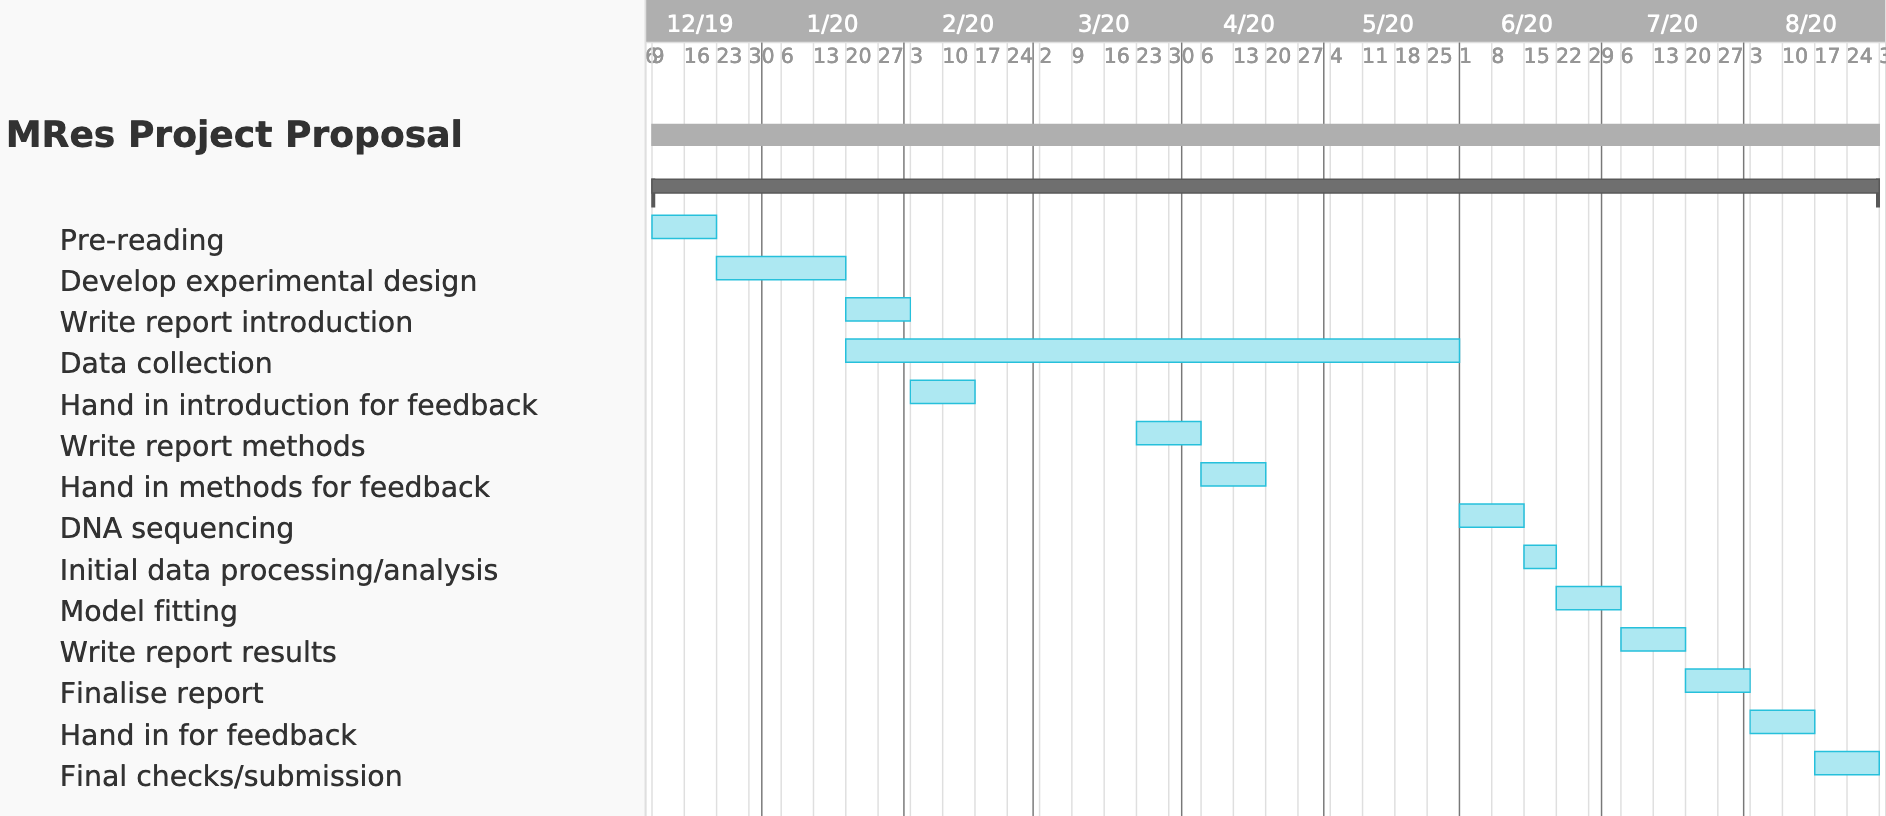
\includegraphics[width=\linewidth]{gantt_chart.png}
	\caption{Gantt chart of proposed project timeline Dec 2019 - August 2020} 
\end{figure}

\section{An itemised budget}
\begin{table}[h!]
  \begin{center}
    \begin{tabular}{l|c|r} % <-- Alignments: 1st column left, 2nd middle and 3rd right, with vertical lines in between
      \textbf{Item} & \textbf{Cost}}\\
      \hline{} 
      16s rDNA sequencing & \pounds15/sample\\
      Containers/substrate for experimental treatments & \pounds200-300\\
      \hline{}
      Request maximum budget & \pounds500\\
    \end{tabular}
  \end{center}
\end{table}

\newpage
  \bibliographystyle{plain}
  \bibliography{DissProp}
 
\newpage
\section{Approval}

I have seen and approved the proposal and the budget.\\
\newline
\newline
\newline
\noindent Name:
\newline
\newline
\newline
\newline
\newline
\newline
\noindent Signature:
\begin{wrapfigure}{r}{17cm}

\includegraphics[width=5cm]{signature.png}
\end{wrapfigure} 
\newline
\newline
\newline
\newline
\newline
\newline
\noindent Date:


  
\end{document}